\chapter{Implementation}

\section{Technical Details}

In this section we outline the general structure and design choices that went into the implementation of this process. 
While we wont go into the minutiae of the source code, it can be found at the GitHub repository...\question{GitHub link?}
The project is primarily implemented using three different frameworks: PyTorch, PyTorch Lightning and Hydra.
PyTorch provides the base deep learning methods, while PyTorch Lightning also provides a bunch of additional features, such as handling of different computational devices such as GPU, handling the different train, validation and test data splits, an extensive callback API and more.
Importantly, PyTorch Lightning also provides encapsulation of the inference process through the use of LightningModules.
A goal for the implementation has been to separate the modelling, the data and the inference methods as much as possible.
This makes it possible to effectively compare different methods of inference across different models and data.
The overall architecture can be seen in \cref{fig:sw-arch}.
\begin{figure}[htbp]
    \centering
    % spellchecker: disable

\begin{tikzpicture}[
    class/.style={rounded corners=0.3cm,minimum height=1cm,fill=blue!50,draw=black},
    back group/.style={rounded corners, draw=black, 
                     dashed, inner xsep=0.2cm, inner ysep=0.3cm, 
                     anchor=west},
    node distance = 1cm, 
    auto
    ]
    \node[class,fill=brightgreen!50] (sgd-module) at (2, 4.75) {SGDInference};
    \node[class,right=0.2cm of sgd-module.east,fill=brightgreen!50] (vi-module) {VariationalInference};
    \node[class,right=0.2cm of vi-module.east,fill=brightgreen!50] (mcmc-module) {MCMCInference};
    \node[class,above=1.2cm of mcmc-module] (sampler) {Sampler};
    \begin{scope}[on background layer]
        \node (inf-modules) [back group] [fit=(sgd-module)(vi-module)(mcmc-module),label={below right:InferenceModule}]{};
    \end{scope}
    \node[class, left=of inf-modules] (data-module) {DataModule};
    \node[class, above=1cm of data-module] (dataset) {Dataset};
    \node[class, align=center, above=2cm of inf-modules] (conv) {Bayesian-\\ConversionConfig};
    \node[class,left=1cm of conv] (model) {Model};
    \path (data-module) -- (mcmc-module) node[midway] (center) {};
    \node[class, below=2.5cm of center, fill=grey] (trainer) {pl.Trainer};
    % \node[class] (8) at (3.5, 7) {Priors};
    \draw [->] (sampler) -- (mcmc-module);
    \draw [->] (model) edge (mcmc-module);
    \draw [->] (model) edge (vi-module);
    \draw [->] (model) edge (sgd-module);
    \draw [->] (conv) edge (mcmc-module);
    \draw [->] (conv) edge (vi-module);
    \draw [->] (conv) edge[dashed] (sgd-module);
    \draw [->] (dataset) -- (data-module);
    \draw [->] (data-module) edge[out=-90, in=90] (trainer);
    \draw [->] (inf-modules) edge[out=-90, in=90] (trainer);
\end{tikzpicture}

    \caption{Overall architecture of inference implementation. }
    \label{fig:sw-arch}
\end{figure}

\subsection{Models}
The models used in this project are defined in the \texttt{src/models} directory.
These are implemented as PyTorch modules with some additional methods that are used by the other components. 
At a high level, they define some amount of trainable parameters $\theta$, as well as a mapping from input $x$ to output $y=f_\theta(x)$. 
They also define an observation model through $p(y|x, \theta)$ using the distribution objects provided by PyTorch.
These model does not provide any probabilistic assumptions about model parameters.
They are instead applied dynamically to each model according some configuration, which allows for 
In practice, for the bayesian methods, each Pytorch module with learnable parameters is changed for a Bayesian copy that also includes information about the parameter priors.

\subsection{Data}
Data is represented by PyTorch datasets.
The dataset abstraction is implemented using two methods, one for getting the total size of the dataset $N$, and another for getting extracting the $i$th observation.
For use with PyTorch Lightning these dataset are then wrapped in a \texttt{pl.LightningDatamodule} object, which defines how the data should be used during training, specifying data splits, batch sizes etc.
For this project, a general \texttt{pl.LightningDatamodule} implementation, \texttt{DataModule} is used in order to reduce code duplication and better be able to ensure consistency between experiments. 

\subsection{Inference Modules}
The inference modules defines the different means of inference and are initialized using a model object.
They are implemented as \texttt{pl.LightningModule}s, and are therefore meant to be used with the \texttt{pl.Trainer} object alongside a \texttt{pl.Datamodule} for model fitting. 
There are three different inference methods implemented: regular stochastic gradient descent, variational inference and inference using Markov chain Monte Carlo inference.

In order to implement probabilistic methods, we have to supply the inference methods with additional information in form prior probabilities of the parameters. 
These are specified using a user specified Bayesian conversion configuration.
We then substitute each module with trainable parameters with a corresponding Bayesian module, which also defines parameter priors, as well a method for calculating the prior log probability.
The dynamical approach is chosen since it makes specifying the models simpler, allows for adjusting the priors dynamically and differently based on the methods in question, and also allows for training of models specified elsewhere like pre-trained models. 
For comparison with the probabilistic methods, the SGD inference optionally allows for using MAP estimation also using this framework.

\subsection{MCMC Inference}

The regular SGD inference also allows for MAP estimation

, for comparison with the other probabilistic methods.

Probabilistic attributes of models such as priors are added dynamically based

\subsection{Variational Inference}
The variational inference module is implemented


\subsection{Samplers}
The different sampler are implemented using a common interface, each 
After initializing each sampler, they are set up by registering to them an object defining what distribution should be sampled from. 
This object, dubbed Samplable, should define the following properties: The current state as a PyTorch tensor, the shape of the state, the logarithmic proportional probability density at the current state, and the corresponding gradient.  

In the context of deep learning inference, the model parameter posterior is represented by a ParameterPosterior object that wraps the model object and allows for setting of different sets of observations.
The wrapper then implements the Samplable interface, with the state being model parameters stacked as single one dimensional tensor, and uses the observation model and autograd to implement the remaining methods.


\section{Simulated Experiments}

In order to verify the implementation of the methods, some simulation experiment out. 
The first experiment is a recreation of an experiment also carried out in the SGHMC paper, where they sample from a bimodal distribution with $\log p(x) \propto 2 x^2 - x^ 4$ with different configurations. 
First, the distribution is sampled from as is, using regular HMC.
Then the batched dynamics in \cref{eq:sghmc-model} are simulated by adding simulated noise $\epsilon \sim \mathcal{N}(0, 4)$ to the gradient during the sampling process. 
The distributional assumptions of SGHMC are thus fulfilled exactly, and we may also use the known noise scale as the noise estimate for SGHMC. 
With this introduced noise we also investigate the naive approach to using HMC, both with and without using an MH step. 
The resulting sampled distributions can be seen in \cref{fig:synthetic}
\begin{figure}[htb]
    \centering
    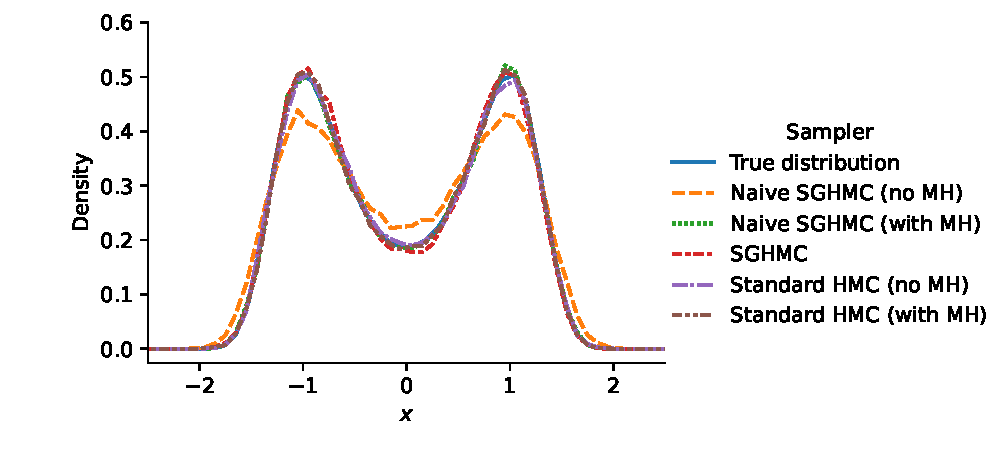
\includegraphics[width=0.9\textwidth]{Figures/synthetic.pdf}
    \caption{Samples from $\log p(x) \propto 2 x^2 - x^ 4$ for different sampling configurations}
    \label{fig:synthetic}
\end{figure}
These result seem to verify our that our implementation is correct.
We also see that the sample distributions from both the standard HMC sampler and the SGHMC sampler closely resembles the true distribution. 
The naive SGHMC sampler does seems to break down when no MH step is included, and since we also compare with regular HMC with no MH step, this demonstrates that it may not be purely down to omitting the MH step. 

If we include an MH step, the naive approach also seem to work, however we are not adding any noise to $E(\cdot)$ when performing the MH step, corresponding to calculating $E(\cdot)$ across the whole data set. 
This is impractical in the context of deep learning, but one could imagine an alternative naive HMC approach where an MH step based on each individual batch of data. 

This experiment also doesn't address whether noise the dynamics of \cref{eq:sghmc-model} are even reasonable as a model for the noise introduced through batching the gradient. 

In order to address these points, we perform an additional simulation experiment. 
This is also to demonstrate the relevance of the different methods in the context of MCMC inference.
We consider the polynomial model of $P(x) = -x + \frac{1}{2}x^2 + \frac{1}{3}x^3$, 
and with $\epsilon \sim \mathcal{N}(0, 1)$, consider a set learning points $y_i = P(x_i) + \epsilon$ for $i=1,\dots,15$, where $x_i$ are linearly spaced over the interval $[-3, 3)$ with a small amount of noise added. 
We then consider the problem of bayesian polynomial regression with known noise $\sigma=1$ and the regression model:
\begin{align*}
    P(x) = a_0 + a_1 x+a_2 x^2 + a_3 x^3
\end{align*}
where each parameter are given a $\mathcal{N}(0, 1)$ prior.
The exact parameter posterior $p(a|x,y)$ for this regression problem is known, and can therefore be compared to the sampled distribution of the samplers. 
More specifically, three sampling strategies are considered, regular HMC conditioned on all data points, HMC where each sample is based on a batch of 5 observations, and SGHMC also with batches of 5 observations.
For demonstration, a plot of the sampled joint distribution of $a_1$ and $a_3$ can be seen in \cref{fig:simulated_joint_comp}.
\begin{figure}[htbp]
    \centering
    \begin{subfigure}[b]{0.4\textwidth}
        \centering
        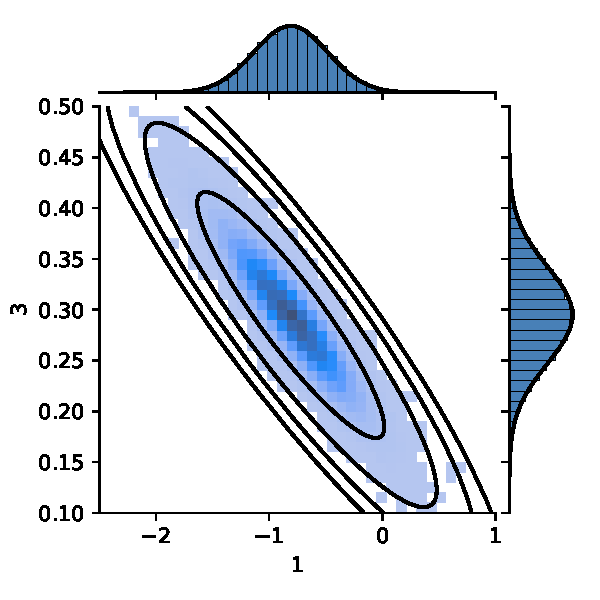
\includegraphics[width=\textwidth]{Figures/simulated_joint_HMC_15.pdf} 
        \caption{HMC conditioned on all data points.}
    \end{subfigure}
    \begin{subfigure}[b]{0.4\textwidth}
        \centering
        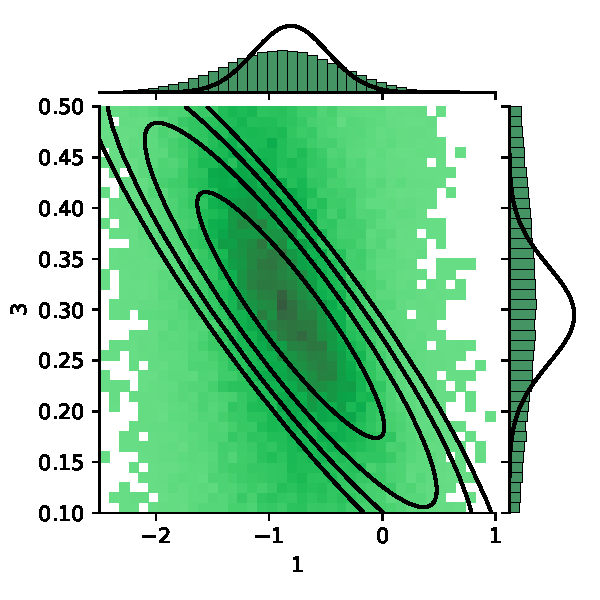
\includegraphics[width=\textwidth]{Figures/simulated_joint_HMC_5.pdf} 
        \caption{HMC with batch size 5}
    \end{subfigure}
    \begin{subfigure}[b]{0.4\textwidth}
        \centering
        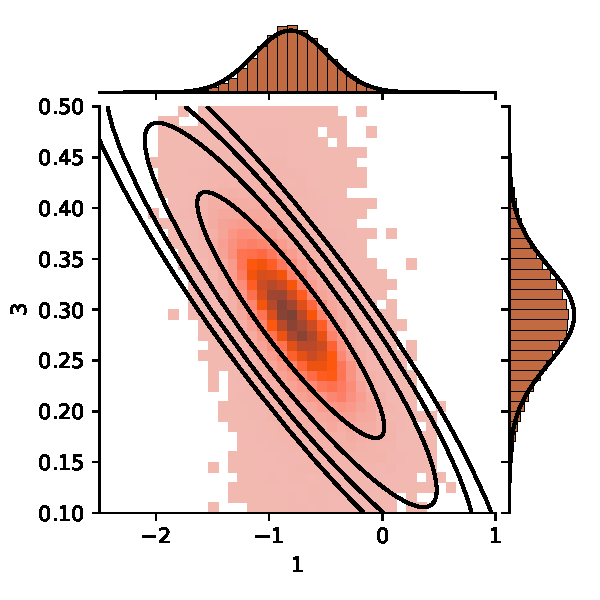
\includegraphics[width=\textwidth]{Figures/simulated_joint_SGHMC_5.pdf} 
        \caption{SGHMC with batch size 5}
    \end{subfigure}
    \caption{Joint distribution of samples for $a_1$ and $a_3$ for the polynomial regression example for HMC and SGHMC for different batch sizes, with the actual posterior density also shown.}
    \label{fig:simulated_joint_comp}
\end{figure}
We find that the also with this approach to the naive SGHMC the batched HMC doesn't, with the sampled posterior having 

with not even the marginal densities being anywhere close to the actual parameter posterior.
Notably, the SGHMC seems to provide a more reasonable estimate, however still with some overdispersion.
In the following section, a possible improvement upon this algorithm is discussed.

